%!TEX root = ../../master.tex
\section{Application vs Infrastructure Level Resilience}
Throughout our work with resilience, we noticed the recurring distinction between application level and infrastructure level resilience. Some measures to improve resilience can be implemented in source code written in e.g. Java and Python. Other measures can be applied at the infrastructure level by handling the applications' surroundings in an intelligent way. Nygard presents several patterns to handle the previously described antipatterns. Some of these patterns will be described and put in the context of application vs. infrastructure level resilience.

\subsection*{Application Level Resilience}
At the application level, software architecture and implementation are in focus. The software is, of course, run in some environment, but the following will describe general improvements of architectures. \\

%!TEX root = ../../master.tex
\noindent \textbf{Use Timeouts}
\\
The timeout pattern is concerned with the first fallacy about trusting the network blindly. The risk of blocking a thread forever and eventually draining a thread pool is present without timeouts. Slow responses can lead to cascading failures and chain reactions. The solution is to limit the acceptable waiting time and have a fallback strategy. Using the terms from Figure~\ref{fig:our_resilience_definition}, this is a way of prioritizing availability over reliability by tolerating a lower level of consistency. A lower level of consistency could be a degradation in the returned content e.g. returning a top10 movie list instead of a personalized list. \\

\noindent \textbf{Circuit Breaker}
\\
A circuit breaker protects a service from an unhealthy integration point by applying rules for when it is allowed to call the integration point. When an integration point fails too many times (e.g. timeout) it is blocked and transitions from the state \textit{closed} to \textit{open} (Figure~\ref{fig:circuit_breaker_states}). Given a configuration, the circuit breaker transitions to the \textit{half-open} state in which it attempts a reset its state to see if the integration point is safe to call again. If the attempt succeeds the state transitions from \textit{half-open} to \textit{closed}, and if the attempts fails it returns to the \textit{open} state.

\begin{figure}[H]
    \centering
    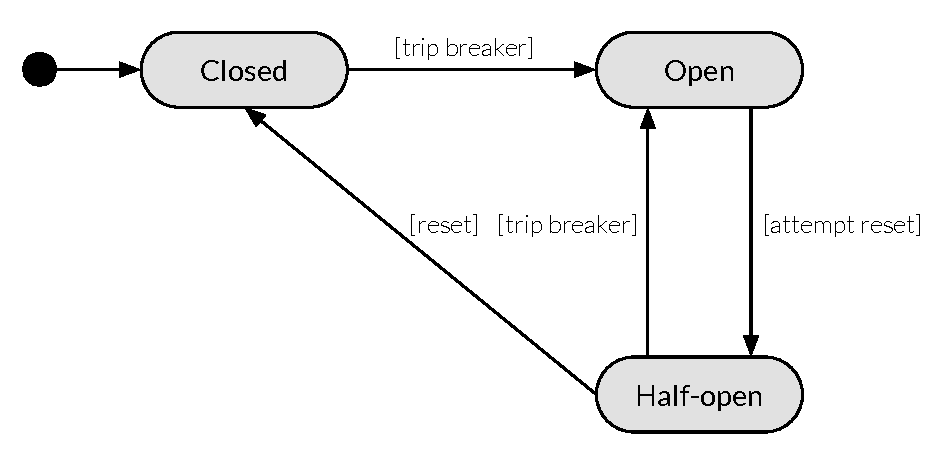
\includegraphics[width=10cm]{figures/circuit_breaker_state_diagram}
    \caption{Circuit Breaker States}
    \label{fig:circuit_breaker_states}
\end{figure}

\noindent 
Fallback methods can be used together with circuit breakers to degrade gracefully instead of failing. As with timeouts, this is trading higher availability at the cost of consistency and reliability. An experiment involving circuit breakers, fallback methods and avoidance of cascading failures is presented in Section~\ref{sec:exp_integration_points}. \\


\noindent \textbf{Fail Fast}
\\
The fail fast pattern summarizes the similarity in the two previous patterns. Failing slowly is worse than failing fast, and several antipatterns are linked to waiting. If services are synchronously chained (A calls B who calls C) much time may be wasted in the form of blocked threads. Timeouts and circuit breakers exemplify how this pattern can be implemented. \\

\noindent \textbf{Bulkheads}
\\
Another recurring theme in the previous patterns has been the containment of damage. In ships, bulkheads are used to contain damage to a certain part of a ship (Figure~\ref{fig:bulkheads}). 

\begin{figure}[H]
    \centering
    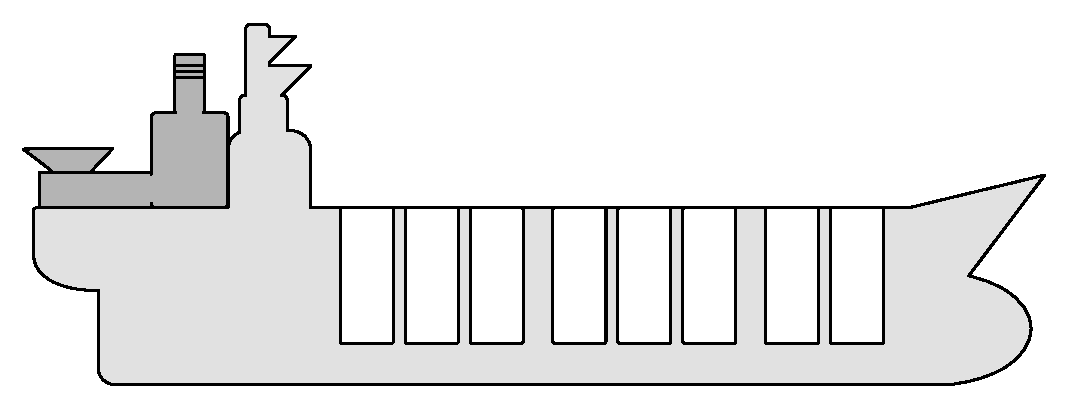
\includegraphics[width=10cm]{figures/bulkheads}
    \caption{Bulkheads}
    \label{fig:bulkheads}
\end{figure}

\noindent
Bulkheads can be applied at different levels. At the application level, the architecture can be split into multiple services such as microservices and gain the containment through multiple processes. 
When interacting with different integration points, different thread pools within the service can be used. The benefit comes with the price of less flexibility to share resources when one of the integration points is passive. \\

\noindent \textbf{Decoupling Middleware}
\\
Nygard describes different degrees of coupling in middleware and points out that some of the previously described problems can be mitigated by decoupling middleware. A step in this direction could e.g. be to choose a message queue instead of HTTP for communication between services.

\begin{citat} []
"Message-oriented middleware decouples the endpoints in both space and time. Because the requesting system doesn't just sit around waiting for a reply, this form of middleware cannot produce a cascading failure."\textbf{- Nygard, 2007} \cite[p. 115]{nygard2007release}
\end{citat}

\noindent Furthermore, Nygard states that synchronous (tightly coupled) middleware's advantage is \textit{"its logical simplicity"} opposite of asynchronous processes that are \textit{"inherently harder"} \cite[p. 115]{nygard2007release}. Newman points out the same increase in complexity in asynchronous programming. The inherent complexity will most likely result in an increase in Mansouri et al's \cite[p. 16]{omer2013resilience} disruption caused by a human factor.

\begin{citat} []
"The associated complexity with event-driven architectures and asynchronous programming in general leads me to believe that you should be cautions in how eagerly you start adopting these ideas." \textbf{- Newman, 2015} \cite[p. 57]{newman2015building}
\end{citat}

\noindent On the other hand, Bonér, the inventor of the Akka framework, expresses asynchronous communication as a requirement for isolation and, thereby, resilience.
\begin{citat} []
Isolation is a prerequisite for resilience and elasticity and requires asynchronous communication boundaries between services to decouple them in: Time (Allowing concurrency), Space (Allowing distribution - and mobility — the ability to move services around) \textbf{- Bonér, 2016} \cite[p. 7]{boner2016reactive}
\end{citat}

\noindent Throughout the rest of this master's thesis, the focus will primarily be on synchronous communication. The designed course (Chapter~\ref{chap:designing_learning_acitivty}) already contains many new concepts. Netflix is an example of a company using a synchronous architecture. However they have created a reactive extension called RxJava that introduces asynchronous behavior.


\subsection*{Infrastructure Level Resilience}
At the infrastructure level, the environment around the application is in focus. The cloud stack described in Figure~\ref{fig:cloud_stack}, from server to runtime, plays an important role when software transitions from developer machines to a production environment. \\

\noindent Docker has decreased the hurdle of recreating the same environment. Encapsulating everything in a lightweight container image assures identical dependencies on developer machines and in the production environment. The hardware and network topology remains different and risk failing in one way or the other. Some of these errors can be handled at the application level, but starting a new process in the environment outside the application requires something from the infrastructure level. \\

\noindent \textbf{Test Harness}
\\
A test harness can help prepare for production in addition to existing tests. It is a way to make the application more robust, and whether it belongs to the application level or infrastructure level resilience can be discussed. The idea is to inject faults in the external network calls in the application by calling a malicious server that simulates network errors. The reaction of the system under test will show whether it is "cynical" enough \cite[p. 111]{nygard2007release}. Netflix uses similar concepts presented later in this chapter. \\

\noindent \textbf{Steady State}
\\
The last Nygard pattern we will present is Steady state which is a pattern for minimizing human fiddling and keeping servers running without intervention. 
\begin{citat} []
Every single time a human touches a server is an opportunity for unforced errors. \textbf{- Nygard, 2007} \cite[p. 100]{nygard2007release}
\end{citat}

\noindent Compared to the previously mentioned human factor, this is about minimizing the risk of the human factor in the production environment. A similar concept is found from continuous integration in which "hurtful" tasks are automated and thereby become less error-prone. The quote behind this is: \textit{"if it hurts, do it more often"} \cite{fowler2011frequencyreducesdifficulty}. This results in a declarative definition of how to perform a challenging task instead of relying on memory. \\

\noindent \textbf{Replication and Redundancy} \\
If a service instance crashes or fails, an action must be taken. In this regard, fault tolerance and redundancy can switch to a backup instance. A resilient reaction when an instance fails is replacing the failed replica (instance) with a new one. By running redundant instances, service failures can be mitigated. \\

\noindent
Replication also serves the purpose of improved performance by adding a horizontal load balancer in front of multiple replicas. In this way, a given workload is distributed across several replicas. The performance can be improved by adding more replicas. \\

\noindent
These mechanisms are obtained at the infrastructure level, and a cluster management system such as Kubernetes can maintain a number of running replicas. In Kubernetes, a desired state can be specified. A control loop then measures the observed state and compares it to the desired state. If the two states are unequal, an action will be triggered to align the two states. In this case, the infrastructure must provide a mechanism for only directing traffic to the 'healthy' replicas. Directing the traffic is related to \textit{rapidity} which refers to how fast an error is identified and an action taken. An experiment in how Kubernetes handles this will be performed in Section~\ref{sec:exp_replication}.\\

\noindent \textbf{Master Election} \\
High availability (HA) systems require resilience. Single point of failure does not harmonize with resilience. When running a cluster management system, such as Kubernetes or Mesos, the concept of a master is used. To ensure availability when a master, for some reason, disappears a strategy to elect a new master is needed. The concept is: the current leader sends out a heartbeat to maintain the position as the leader while several candidates race to become the leader \cite{kubernetesio}. The difficult part is reaching consensus, and several tools such as ZooKeeper, etcd and Consul exist for this purpose. We will not focus more on this topic throughout the thesis, but it is an important part of ensuring high availability. 